\subsection{Camera Type}
\label{ss:cam_type}
If an object is to be tracked by a laser, the position of the object has to be obtained by camera units as described in \cref{sec:base_setup}. This section presents two different types of cameras that could be used in this project and the pros and cons of each possibility.

One possible camera that can be used for the system is the Microsoft Kinect. This camera also provides other features, some of which could be useful for the project, such as built-in body motion tracking, depth sensors and night vision\cite{kinect}. The motion tracking and depth sensors can be used to obtain the intruders position and the dark vision makes it possible to track objects regardless of the light intensity. One issue of the Kinect is the retail price as it costs 1199 DKK\cite{kinect_price}. To have full coverage of a room it can be necessary to use several Kinects. This is because the room could be too big or that there are objects, such as furniture, which results in blind spots for the Kinect. The effect of using the Kinect is therefore an increase in cost for the system in exchange of having the additional functionality of the Kinect.

\begin{figure}[ht]
  \centering
  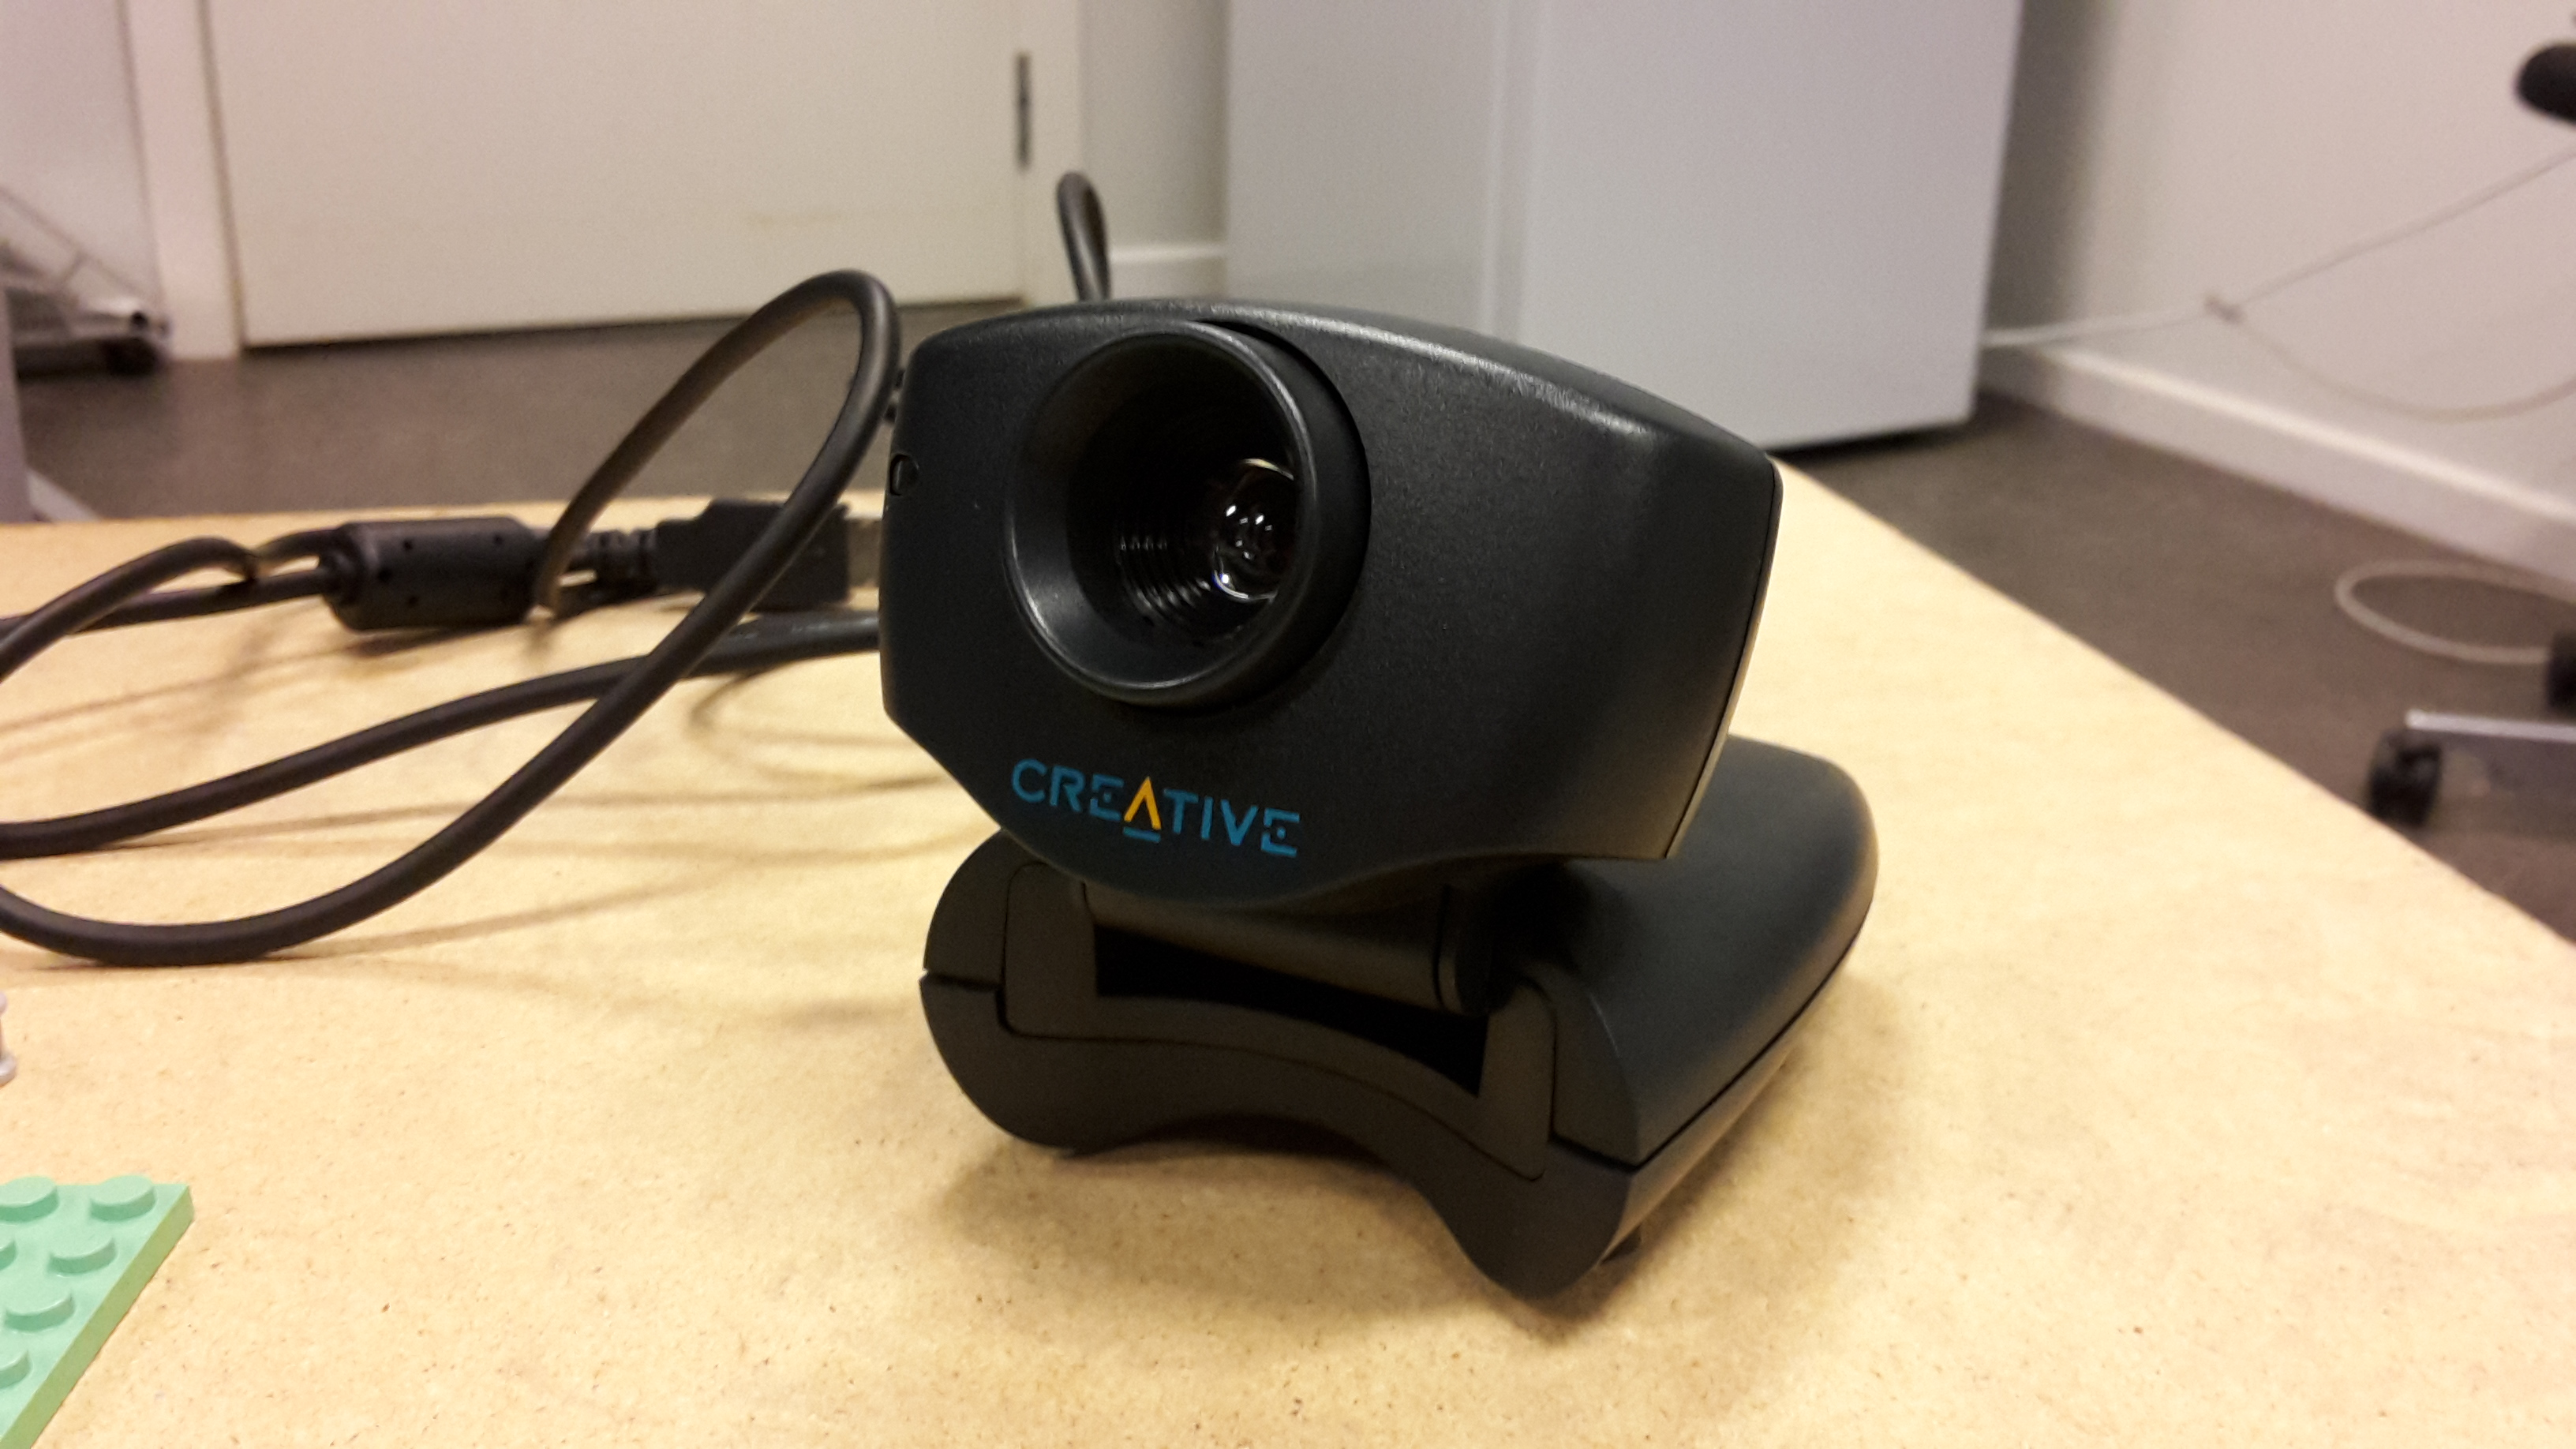
\includegraphics[scale=0.1]{graphics/cvbw3.jpg}
  \caption{\gls{cvbw3} chosen for the project.}
  \label{fig:cvbw3}
\end{figure}

An alternative solution is having webcams with no functionality aside from providing a stream of 2D images. The stream of images can be used to get the direction of the object relative to the respective webcam. To achieve a similar functionality as the first solution with respect to the ability of calculating the depth of an object, it will be necessary to use more than one webcam to triangulate an objects position. An example of a webcam that provides this functionality is the \acrfull{cvbw3}\cite{video_blaster}, which is illustrated in \cref{fig:cvbw3}, but any webcam with the functionality of providing a stream of 2D images will do. The major advantage of this solution is the price; a cheap consumer webcam bought at a Danish retailer is estimated to be around 150 DKK, as seen on price comparison sites\cite{pricerunner_webcam}\cite{ebd_webcam}.

The project has been offered six \acrfull{cvbw3}\cite{video_blaster}, which afford the required functionality while also being relatively old, as they are produced in 1999. In this sense the project also serves to show the possibility of using newer webcams that are equally or more sophisticated in terms of point of view and resolution. This offer was accepted since the cameras have the desired functionality. A consequence of this choice is that the \gls{cvbw3} communicates over USB, which limits what devices that can be used to analyse the image stream.